%!TeX root=main.tex
\chapter{مروری بر کار‌های مرتبط}
\thispagestyle{empty}

برای حمله به شبکه‌های عصبی، می‌توان شبکه‌های عصبی عمیق در معرض نمونه‌های تقابلی قرار داد و با آموزش تقابلی، مقاومت
\LTRfootnote{Robustness}
و نیرومندی شبکه را افزایش داد. از روش‌های ارائه شده برای حمله می‌توان به روش‌های زیر اشاره کرد:
\begin{itemize}
	\item
	علامت‌ی گرادیان سریع
	\LTRfootnote{Fast Gradient Sign Method (FGSM)} \cite{Goodfellow2015ExplainingAH}, \cite{Kurakin2017AdversarialEI}
	
	\item
	روش کاهش گرادیان تصویر شده 
	\LTRfootnote{Projected Gradient Descent (PGD)} \cite{Kurakin2017AdversarialML}
	
	\item
	حمله کارلینی و وگنر
	\LTRfootnote{Carlini and Wagner Attack (C\&W)} \cite{Carlini2017TowardsET}
	
	\item
	حمله تک پیکسل
	\LTRfootnote{One pixel attack} \cite{Su2019OnePA}
	
	\item
	روش تکرار شونده پایه
	\LTRfootnote{Basic Iterative Method (BIM)} \cite{Kurakin2017AdversarialEI}
	
	\item
	روش فریب عمیق
	\LTRfootnote{DeepFool} \cite{MoosaviDezfooli2016DeepFoolAS}
\end{itemize}
در ادامه به توضیح الگوریتم علامت گرادیان سریع پرداخته ‌می‌شود.

\section{الگوریتم علامت گرادیان سریع}
یکی از روش‌هایی که برای آموزش تقابلی موثر ارائه شده است، روش علامت گرادیان سریع است 
\cite{Goodfellow2015ExplainingAH}
که به صورت بهینه‌ای یک دستکاری تقابلی برای یک تصویر را محاسبه می‌کند.
\\
این روش جزو حمله‌های جعبه سفید است زیرا حمله‌کننده
\LTRfootnote{Adversary}
نیاز دارد که به معماری و پارامتر‌های مدل در تمام زمان دسترسی داشته باشد.

\subsection{معادله} 
معاله‌ی الگوریتم علامت گرادیان سریع به صورت زیر است: 
\begin{equation} \label{eq:fgsm}
	X^{adv} = X + \epsilon \cdot sign(\nabla_XJ(X, Y_{true}))
\end{equation}
در معادله
\ref{eq:fgsm} 
داریم:
\begin{itemize}
	\item $X$
	، تصویر اصلی و دست‌نخورده
	\item $X^{adv}$
	، نمونه تقابلی که پس از اعمال دستکاری و اجرای روش نشانه‌ي گرادیان سریع بر روی تصویر اصلی بدست می‌آید
	\item $\epsilon$
	 ، یک ثابت براي تعیین شدت حمله (بزرگی آشتفگی تقابلی)
	\item $J$
	 ، تابع زیان
	\item $Y_{true}$
	، دسته و برچسب صحیح تصویر اصلی
	\item $\nabla_X$
	، شیب تابع هزینه
\end{itemize}

در این معادله
(\ref{eq:fgsm}) 
، هر چه مقدار $\epsilon$ بیشتر باشد، نمونه‌ تقابلی نسبت به تصویر اصلی غیر قابل تشخیص‌تر می‌شود.

\subsection{عملکرد الگوریتم}

در این روش هدف این است که یک نویز محاسبه شده که تصادفی نیست و در راستای شیب تابع هزینه، در تصویر اصلی وجود دارد، را به تصویر اولیه اضافه کند. 
در این روش حمله‌کننده دقیقا از روشی که برای آموزش شبکه در تشخیص مرز‌های دسته‌بندی استفاده می‌شود، بهره می‌برد به این طریق که تصویر دستکاری شده را طوری تنظیم می‌کند که تابع زیان به سمتی هدایت شود که با تصویر دیگری اشتباه گرفته شود.
\\
روش الگوریتم علامت گرادیان سریع برای مدل‌های خطی بهترین حمله طبق قاعده
$L^{\infty}$
است و از‌ آن‌جایی که شبکه‌های عصبی مدل‌هایی غیر خطی هستند، به این نتیجه‌ می‌توان رسید که در مقابل شبکه‌های عصبی چندان خوب نمی‌تواند عمل کند.

\subsection{یک مثال از نمونه تقابلی}
همان طور که در شکل 
\ref{fgsmEx}
‏مشاهده می‌شود، یک نمونه از تصویر‌های مجموعه داده‌ی ‌ImageNet  که بر روی شبکه GoogLeNet آموزش دیده است، آورده شده است که شبکه با اطمینان
\lr{۵۷.۷٪} 
تصویر را پاندا تشخیص می‌دهد. سپس با اضافه کردن بردار بسیار کوچکی به تصویر می‌توان طبقه‌بندی شبکه را به خطا انداخت. مشاهده می‌شود که مدل، تصویر دستکاری شده را یک میمون درازدست با اطمینان
\lr{۹۹.۳٪}
تشخیص داده است.
\begin{figure}[H]
\center{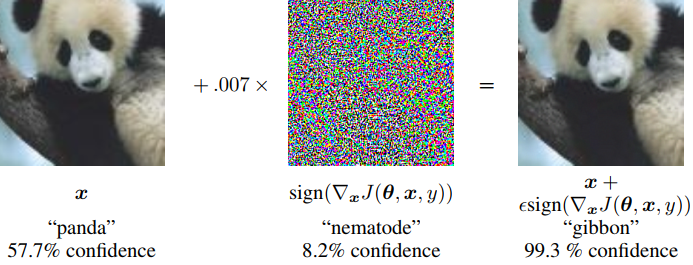
\includegraphics[width=\linewidth]{images/fgsmEx.PNG}}
\caption{نمونه‌ای از اعمال الگوریتم علامت گرادیان سریع
	\cite{Goodfellow2015ExplainingAH}}
\label{fgsmEx}
\end{figure}
